\begin{figure}[H]
    \centering
    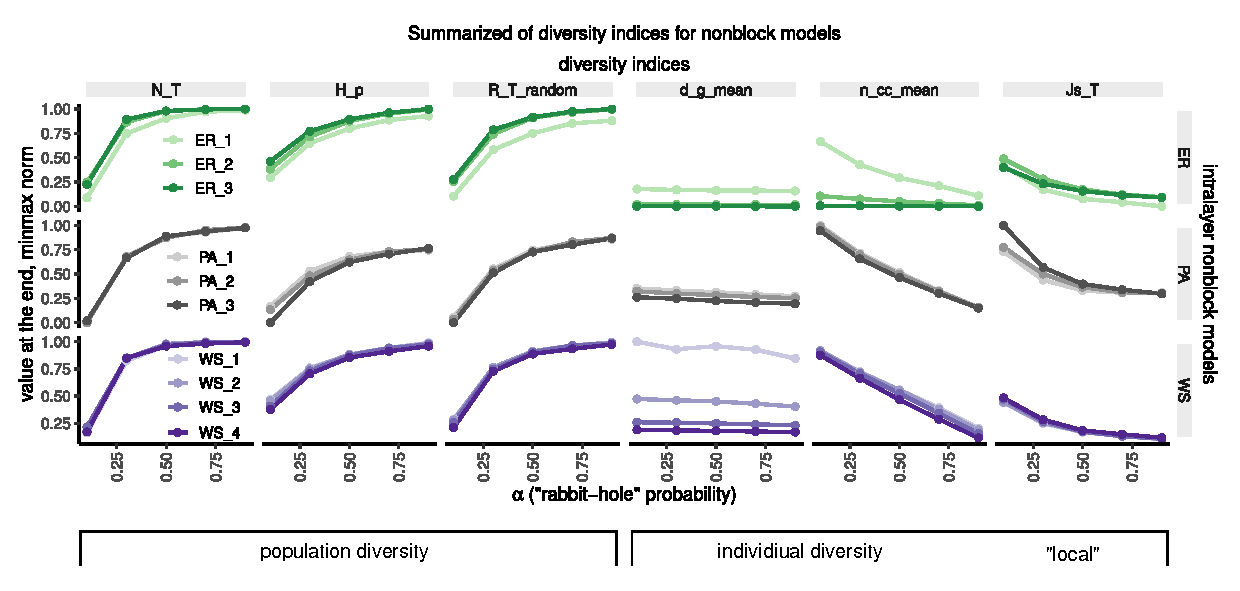
\includegraphics[width=0.95\textwidth,center]{../figures/report/Fig4.pdf}
    \caption{\label{fig:4}
    \textit{Summary of population and individual diversity indices due to $\alpha$, across different nonblock models (with random initialization)}. The values here are at the end of the simulation, and min-max normalized within each metric (panels from left to right, see text and \autoref{fig:3} for description of these different definitions). The different models are shown by colors and panels from top to bottom (see also \autoref{fig:2} for correspondence of colors).
    }
\end{figure}